\documentclass[conference]{IEEEtran}
\IEEEoverridecommandlockouts
\usepackage{cite}
\usepackage{amsmath,amssymb}
\usepackage{booktabs}
\usepackage{tabularx}
\PassOptionsToPackage{hyphens}{url}\usepackage{url}
\usepackage{tikz}
\usepackage{pgfplots}
\usetikzlibrary{patterns}
\usepackage{microtype}
\usepackage{balance}
\usepackage[hidelinks]{hyperref}
\pgfplotsset{compat=1.16}
\newif\ifanonymous
\anonymoustrue
\ifanonymous
  \hypersetup{pdftitle={Gaming ISO 20022 Payment Messages: A Temporal Adversarial Benchmark for Purpose Codes, Party Fields, and Message Paths},pdfauthor={Anonymous}}
\else
  \hypersetup{pdftitle={Gaming ISO 20022 Payment Messages: A Temporal Adversarial Benchmark for Purpose Codes, Party Fields, and Message Paths},pdfauthor={Abhishek Sharma}}
\fi
\begin{document}
\title{Gaming ISO~20022 Payment Messages:\\
A Temporal Adversarial Benchmark for\\
Purpose Codes, Party Fields, and Message Paths}
\ifanonymous
\author{\IEEEauthorblockN{Author names withheld for double-blind review}
\IEEEauthorblockA{Affiliations withheld for double-blind review}}
\else
\author{\IEEEauthorblockN{Abhishek Sharma}
\IEEEauthorblockA{\textit{Senior Member, IEEE}\\
Independent Researcher\\
abhishek.sharma@ieee.org}}
\fi
\maketitle
\begin{abstract}
ISO~20022 gives payment controls structured data, but message creators still
decide where names, addresses, and purpose information appear. We study
\emph{message gaming}: deliberate edits to purpose codes, party fields, or the
message path that lower a modelled alert probability while preserving the
payment's economic meaning. A seeded generator gives each debtor--creditor
pair latent behaviour and emits pain.001 and pacs.008 records in time order
with a controlled rate of ordinary defects. A cost-bounded evader applies up
to two of eleven manipulations. Every message is schema-valid and every edit
preserves its stated invariants. Every evaluation is temporal: the earliest
60\% of a run trains, the next 20\% freezes alert thresholds, and the latest
20\% is scored, with pair-clustered bootstrap intervals over ten seeds.
Screening-evasion lift (SEL) is measured as a paired counterfactual on each
manipulated payment. At a frozen 1\% alert threshold, where at most
22.4\% of gamed messages can be recovered, the best supervised model
recovers 18.0\% and falls from AUC 0.633 to 0.490 on a
withheld misfielding family; the strongest label-free message-level detector
recovers 3.3\%. A pre-registered test finds that neither the
P1/P2/P3 family ($R^2=0.35$, exact $p=0.125$) nor whether an
edit leaves an internal contradiction ($R^2=0.04$, $p=0.567$)
explains which primitives that model recovers. What separates the families
is the evidence required: on withheld path and structure edits every
message-level detector is at or below chance, while a history-only control
reaches AUC 0.851. Splitting a payment raises per-message lift to
1.44 but lowers attempt-level lift to 0.94 once every child
is screened. Results are synthetic and relative to a published screening
abstraction.
\end{abstract}
\begin{IEEEkeywords}
ISO~20022, payment data quality, purpose codes, sanctions screening,
anti-money laundering, adversarial evaluation, synthetic benchmark
\end{IEEEkeywords}

\section{Introduction}
A payment message is both an instruction and a compliance record. Names,
addresses, amounts, and purpose information feed sanctions, fraud, and
anti-money-laundering controls, and ISO~20022 makes that information easier
to parse. Structure does not remove discretion, though. A message creator
still chooses which optional fields to populate, which purpose code to
declare, how much detail to place in free text, and sometimes which path a
payment takes. Screening is selective by design: Swift's guiding principles
identify the elements that normally warrant direct screening and let other
fields provide context~\cite{swiftgp2021}. Market-practice guidance
records that purpose codes are often misunderstood or placed in the wrong
field~\cite{pmpg2024}. The structured-address requirement that CBPR+ had
scheduled for 14 November 2026 was deferred by Swift in August 2026 after a
community request, with revised timing under consultation~\cite{swift2026ext}.
CPMI's harmonised requirements remain guidance rather than a
mandate~\cite{cpmi2026}. Unstructured and half-structured data will therefore
coexist with structured data for years, and an ordinary data-quality error
and a deliberate low-scrutiny choice can leave the same evidence.

That overlap creates an evaluation problem. A detector can look good by
finding malformed records, even though malformed records are mostly benign.
It can earn a high AUC by learning the edit signatures of one generator, then
fail on a manipulation absent from training. And it can be evaluated with
future information leaking into its history features. The question that
matters operationally is narrower: at an alert capacity a payment operation
could actually run, with thresholds frozen before the scored period, do
deliberate changes remain distinguishable from routine error?

The contributions are eleven message-level manipulations with actors,
costs, and stated invariants, all schema-valid; a generator with pair
behaviour and time order; a temporal protocol with frozen thresholds and
pair-clustered uncertainty; paired counterfactual SEL, which needs no
separate control group; a pre-registered test of what predicts
detectability; and a history-only positive control. Detectors are
conventional on purpose. No real payment, customer, or institution data is
used.

\section{Related Work and Gap}
Public AML resources model who pays whom, how much, and when: the Elliptic
data set~\cite{weber2019}, AMLSim~\cite{suzumura2021},
AMLworld~\cite{altman2023}, SAML-D~\cite{oztas2023}, and the recent AMLgentex
and Tide generators with partial observability and configurable
prevalence~\cite{ostman2025,beukel2026}. None encodes the internal placement
of ISO~20022 fields, so none can express a manipulation whose mechanism is
that a name, code, or narrative sits in a different element. Adversarial
machine learning on tabular financial data is the closest methodological
line: imperceptible tabular perturbations~\cite{ballet2019}, attacks on
imbalanced fraud data~\cite{cartella2021}, and constrained attacks and their
benchmark~\cite{simonetto2022,simonetto2024}. Those attacks move numeric
features under a norm or constraint set; the edits here are discrete,
semantics-preserving message operations whose cost is operational, in the
classical cost-bounded evasion setting~\cite{bruckner2011,biggio2013}. Noisy
payment-address parsing in real traffic~\cite{hammami2024} is the
ordinary-error half of the same overlap. Transaction-purpose
classification~\cite{busson2023} enriches naturally occurring labels rather
than detecting strategically chosen ones. No prior benchmark combines
message-level field operations with a controlled accidental-error floor and
a temporal, capacity-constrained evaluation.

\section{Threat Model and Manipulations}
The adversary can construct or amend a payment instruction but controls
neither the screening system nor its threshold. A black-box adversary knows
public guidance and receives a coarse accept-or-hold outcome; its admissible
set excludes the targeted code substitutions P2a, P2b, and P2d. A grey-box
adversary also knows the relative ordering of the benchmark's purpose-code
weights. Route choice (P3a) is a per-record capability held by a PSP,
bank-side actor, or multi-channel originator, drawn for 30\% of
illicit records. Let $x$ be an illicit instruction, $m$ an admissible
modification with operational cost $c(m)$, and $\pi(x)$ the alert probability
in the published screening abstraction. The evader chooses
$m^*=\arg\min_m\{\pi(m(x))+\lambda c(m)\}$ subject to $V(m(x))$ and $|m|\le
k$, sampling among improving subsets with a softmax of temperature $T$. $V$ is
checked on every record. Amount, currency, debtor and creditor countries, and
the economic originator and beneficiary are unchanged by every primitive.
P3a changes the path of a single-transaction payment, P3b its decomposition
into children that sum to the amount, and P3c the represented party chain,
where an intermediary replaces the ultimate-party element. Primitives that
need an element the record lacks are inadmissible for that record.

\begin{table}[!t]
\caption{The eleven primitives with actor, cost $c(m)$, and the
pre-registered contradiction label (C: the edit makes two elements of the
message, or an element and the creditor's profile, inconsistent).}
\label{tab:prims}
\centering
\scriptsize
\setlength{\tabcolsep}{3pt}
\begin{tabularx}{\columnwidth}{@{}lXcc@{}}
\toprule
ID & Operation (actor: originator or PSP unless stated) & $c$ & C \\
\midrule
P1a & move the ultimate-party name into remittance text & 0.30 & \\
P1b & true town and country into a free-text line; TwnNm set to another town & 0.25 & \checkmark \\
P1c & truncate the listed party's name to four characters & 0.15 & \\
P1d & omit the ultimate debtor & 0.20 & \\
P2a & replace the purpose code by the lowest-weight plausible code & 0.05 & \checkmark \\
P2b & replace the category purpose & 0.08 & \checkmark \\
P2c & omit the purpose code & 0.04 & \\
P2d & declare a salary purpose over a goods or invoice narrative & 0.10 & \checkmark \\
P3a & same single payment on the other path (actor with route choice) & 0.45 & \\
P3b & multiply the file's child count by 3 to 7, children sum to the amount & 0.35 & \\
P3c & an intermediary replaces the ultimate-party element & 0.55 & \\
\bottomrule
\end{tabularx}
\end{table}

Table~\ref{tab:prims} lists the primitives. Whether the P1/P2/P3 family or
the contradiction label predicts detectability was fixed as a question, with
labels and tests, before the first full-scale run (Section~\ref{sec:ct}).

\section{Benchmark and Protocol}
\subsection{Generator}
A run draws $n/20$ debtor--creditor pairs with volume weights from a
Dirichlet distribution. Each pair has a creditor industry and a purpose
profile drawn around the industry's profile, a preferred path
(pain.001 versus pacs.008), and a batching habit with a typical file size. It
also has a party-chain pattern (the ultimate names it uses and how often one
appears), an amount scale, and fixed names and addresses. Messages are emitted in time
order by sampling pairs by weight; each carries its index as timestamp. A
fraction $\eta$ receives one ordinary defect (purpose text in remittance,
partial address destructuring, absent ultimate party, absent category
purpose, in the mix 35/30/20/15\%). A fraction $\rho$ is illicit: the listed
party is the ultimate debtor or the debtor, and the evader edits the record.
Benign remittance text and party names have variable length, so no edit
leaves a length that benign traffic does not show; an audit checks this on
every run. Records serialise to pain.001.001.09 or pacs.008.001.08. Every instance
in the seed-7 test window, every gamed record, and every original was
validated against the official XSDs (100.0\% of 56{,}241
valid), and every gamed record passed its invariant check
(0 violations). Full distributions are in the supplement.

\subsection{Screening abstraction}
A name leg matches listed names against the elements the current path
screens: debtor, creditor, and ultimate-party names on pain.001, debtor and
creditor names only on the interbank leg. For an illicit record whose listed
name sits in a screened element it alerts with probability $P_{\mathrm{name}}$,
reduced to $0.39P_{\mathrm{name}}$ when the name is truncated. A score leg
combines purpose weight $w_p$ (0.08 to 0.45), corridor weight $w_c$ (0.05 to
0.40), amount, and completeness,
\begin{equation}
 s=w_p+w_c+0.2\min(1,\,a/(n_{\mathrm{ch}}\cdot 250{,}000))+0.10\,u+0.08\,t,
 \label{eq:score}
\end{equation}
where $a$ is the payment amount, $n_{\mathrm{ch}}$ the number of children, $u$
indicates a missing ultimate debtor and $t$ a missing town or country; only
the amount term is diluted by splitting. The leg alerts with probability
$p_{\mathrm{score}}=1/(1+e^{-8(s-\tau)})$. A residual floor $f=0.10$ represents
controls outside the evader's reach. Per message,
$\pi=1-(1-p_{\mathrm{name}})(1-p_{\mathrm{score}})(1-f)$; per attempt, the
name leg and floor act once and the score leg once per child, so
$\pi_{\mathrm{att}}=1-(1-p_{\mathrm{name}})(1-f)(1-p_{\mathrm{score}})^{n_{\mathrm{ch}}}$.
The evader optimises the per-message form. Baseline survival is split
between the legs by a name share $\sigma$; the main setting $\pi_0=0.45$,
$\sigma=0.6$ solves to $P_{\mathrm{name}}=0.337$, $\tau=0.782$. Weights
are illustrative constants, not any institution's rule set.

\subsection{Features, detectors, protocol}
Message-level features are the consistency checks C1 (code not in list), C2
(town or country missing, address token in free text), C3 (purpose
implausible for the creditor's industry, ultimate debtor absent), and C4
(salary code over a goods narrative). Completeness and length auxiliaries
complete the vector.
History features use only the pair's strictly earlier messages: purpose
novelty (C5), path novelty, split-count deviation, ultimate-party novelty and
presence deviation, and amount deviation. No label enters any feature. $D_1$
is the fixed rule $\mathrm{C1}+0.5\,\mathrm{C2}+\mathrm{C3}+1.5\,\mathrm{C4}$.
$D_2$ is a gradient-boosted classifier and $D_6$ a logistic regression on
one-hot codes, corridor, amount, and completeness. Both train on gaming
labels. $D_5$ is a local outlier factor on the message-level features of
benign training rows~\cite{breunig2000}. $D_3$ (isolation forest) and $D_4$
(rules plus forest) are in the supplement. $D_7$ is the history-only positive
control, the standardised sum of the six history deviations. No
hyperparameter is tuned on the benchmark.

Each run has $n=200{,}000$ records. The earliest 60\% trains every learned
detector. On the next 20\% the score threshold for each alert capacity (1\%
and 0.1\%) is frozen, with a label-blind fraction for tied scores. The latest
20\% is the test window on which every number below is computed. Gamed
records are 4.5\% of the test window, so no detector can recover
more than 22.4\% at 1\% capacity. We report AUC, average precision
(AP), and recovery and precision at the frozen threshold, as means over ten
seeds with between-seed standard deviations, and pair-clustered bootstrap
intervals within each test window. SEL is paired. Each gamed test record
contributes its original $x$ and edited $m(x)$, both scored by the same
detector with the same prior history, and
$\mathrm{SEL}=\sum(1-\pi_m)/\sum(1-\pi_0)$. Residual SEL multiplies each
term by one minus the frozen alert decision. Leave-one-family-out retrains
$D_2$ and $D_6$ without one family (at $k=1$, pure-family records).

\section{Results}
\begin{table}[!t]
\caption{Test-window results, mean $\pm$ between-seed s.d. over ten runs of
200{,}000 records. Rec.\ and Prec.\ are at the threshold frozen on the validation
window at 1\% capacity; the widest pair-clustered 95\% half-interval for Rec.\
is 0.020. $^\dagger$trains on gaming labels.}
\label{tab:main}
\centering
\scriptsize
\setlength{\tabcolsep}{2pt}
\begin{tabular}{@{}lcccccc@{}}
\toprule
Detector & AUC & AP & Rec.@1\% & Prec.@1\% & Alerts/hit & Rec.@0.1\% \\
\midrule
$D_1$ rules & 0.771$\pm$0.004 & 0.321 & 0.112$\pm$0.005 & 0.499 & 2.0 & 0.022 \\
$D_5$ LOF & 0.775$\pm$0.005 & 0.249 & 0.033$\pm$0.005 & 0.136 & 7.5 & 0.012 \\
$D_7$ history & 0.717$\pm$0.006 & 0.123 & 0.035$\pm$0.004 & 0.205 & 4.9 & 0.003 \\
$D_2$ GBM$^\dagger$ & 0.886$\pm$0.008 & 0.498 & 0.180$\pm$0.014 & 0.818 & 1.2 & 0.021 \\
$D_6$ logistic$^\dagger$ & 0.862$\pm$0.009 & 0.436 & 0.155$\pm$0.013 & 0.712 & 1.4 & 0.020 \\
\midrule
Capacity ceiling & -- & -- & 0.224 & 1.000 & -- & 0.022 \\
\bottomrule
\end{tabular}
\end{table}

\subsection{Recovery at a frozen threshold}
Table~\ref{tab:main} separates ranking from operational recovery under a
threshold frozen before the scored period. Gamed records are 4.5\% of
the test window, so 1\% capacity can recover at most 22.4\%. The
fixed rules $D_1$ recover 11.2\% at precision 0.499: one
alert in two is a gamed message. The local outlier factor $D_5$ has the best
label-free AUC (0.775 against 0.771 for $D_1$) and the second-best
AP, yet the lowest label-free recovery, 3.3\%; the history-only
control $D_7$ recovers 3.5\%. Among label-free detectors neither
AUC nor AP orders recovery at the frozen threshold. The supervised $D_2$
reaches AUC 0.886 and recovers 18.0\%
(80\% of the ceiling, precision 0.818); logistic
regression on the same inputs recovers 15.5\%. Realised alert
rates on the test window stay within 0.002 of the 1\% target, so the
frozen thresholds transferred across the window boundary. The exact
top-1\% ranking metric differs from frozen-threshold recovery by at most
0.011 (supplement). Between-seed standard deviations are at most
0.009 for AUC and 0.014 for recovery.

\subsection{Generalisation, history, and shift}
\begin{table}[!t]
\caption{Left: leave-one-family-out AUC on pure-family test records ($k=1$,
ten seeds; in $\rightarrow$ out for the retrained supervised models,
single value for label-free ones). Right: generator shift, detectors fitted
and thresholds frozen on configuration A, scored on B's test window (three
seeds); B$\rightarrow$B in parentheses.}
\label{tab:loo}
\centering
\scriptsize
\setlength{\tabcolsep}{2pt}
\begin{tabular}{@{}lccc|ccc@{}}
\toprule
 & P1 & P2 & P3 & AUC A$\rightarrow$B & Rec.@1\% & Alert rate \\
\midrule
$D_1$ & 0.551 & 0.825 & 0.383 & 0.730 (0.730) & 0.139 & 0.017 \\
$D_5$ & 0.514 & 0.834 & 0.538 & 0.765 (0.786) & 0.019 & 0.006 \\
$D_7$ & 0.576 & 0.715 & 0.851 & 0.697 (0.702) & 0.035 & 0.007 \\
$D_2$ & 0.633$\rightarrow$0.490 & 0.976$\rightarrow$0.641 & 0.550$\rightarrow$0.502 & 0.875 (0.897) & 0.375 & 0.045 \\
$D_6$ & 0.591$\rightarrow$0.482 & 0.964$\rightarrow$0.677 & 0.543$\rightarrow$0.525 & 0.869 (0.879) & 0.336 & 0.034 \\
\bottomrule
\end{tabular}
\end{table}
Table~\ref{tab:loo} (left) retrains the supervised models without one
family and scores pure-family test records. With P1 withheld, $D_2$ falls from
0.633 to 0.490 (between-seed s.d.\ 0.018), and no
label-free detector exceeds 0.598 on P1, whose records are dominated
by name truncation. The inversion behind the low supervised score is
systematic. In the reduced training window an absent ultimate debtor is more
common among benign records (27\%) than among the remaining
gamed ones, and the gamed rate given absence is 1.1\% against
2.6\% given presence. The two P1 edits that remove the
ultimate debtor therefore score 0.222 (P1a) and 0.210
(P1d) against benign traffic, while truncation, which leaves it in place,
scores 0.568. With P2 withheld the supervised drop is
0.976$\rightarrow$0.641 while the label-free $D_1$ and $D_5$
stay at 0.825 and 0.834. P3 is the pre-registered contrast. Every
message-level detector is at or below chance (0.383 to 0.538; the
withheld $D_2$ 0.502), and the history-only $D_7$ reaches 0.851.
Path substitution, decomposition, and party-chain changes leave the message
coherent but break the pair's prior pattern. Table~\ref{tab:loo} (right) fits the detectors and freezes thresholds on
configuration A, then scores configuration B, whose pair behaviour, industry
and corridor mix, defect composition, batching, and string lengths all
differ. Rankings transfer: every AUC is within 0.022 of its
B$\rightarrow$B value. Thresholds do not: $D_2$'s A-frozen threshold alerts
4.5\% of B's test window instead of 1\%, which is why its
recovery rises to 37.5\% at precision 0.365,
while $D_5$'s alerts 0.6\% and recovers
1.9\%. A capacity budget therefore needs recalibration on
the target traffic even when the ranking model does not. At 0.5\% prevalence
(supplement), precision at the frozen threshold falls to
0.080 for $D_2$ and 0.114 for $D_1$, so the
fixed rules overtake the supervised model, at 13 and
9 alerts per detected manipulation.

\subsection{Paired screening-evasion lift}
\begin{figure}[!t]
\centering
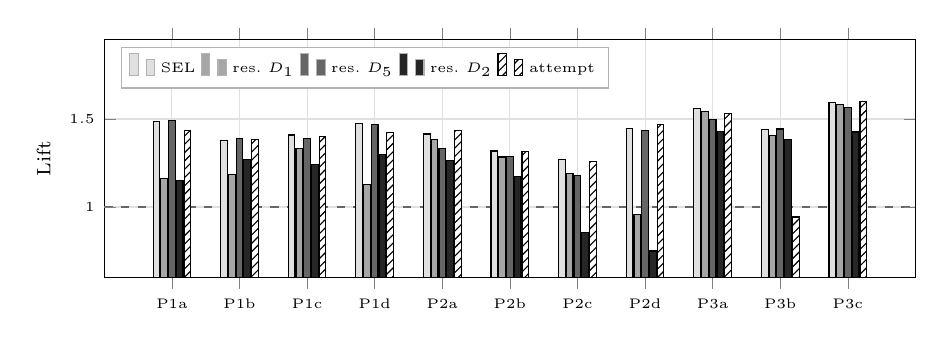
\begin{tikzpicture}
\begin{axis}[
  width=0.98\columnwidth,height=4.6cm,
  ybar=0.4pt,bar width=2.4pt,ylabel={Lift},
  symbolic x coords={P1a,P1b,P1c,P1d,P2a,P2b,P2c,P2d,P3a,P3b,P3c},
  xtick=data,ymin=0.60,ymax=1.95,grid=both,grid style={black!12},
  legend style={at={(0.02,0.97)},anchor=north west,font=\tiny,draw=black!30,legend columns=5},
  label style={font=\scriptsize},tick label style={font=\tiny},
  extra y ticks={1.0},extra y tick labels={},extra y tick style={grid=major,grid style={black!60,dashed}}
]
\addplot[fill=black!12] coordinates {(P1a,1.485) (P1b,1.376) (P1c,1.409) (P1d,1.472) (P2a,1.415) (P2b,1.318) (P2c,1.272) (P2d,1.444) (P3a,1.559) (P3b,1.442) (P3c,1.593)};
\addlegendentry{SEL}
\addplot[fill=black!35] coordinates {(P1a,1.160) (P1b,1.183) (P1c,1.333) (P1d,1.128) (P2a,1.385) (P2b,1.284) (P2c,1.189) (P2d,0.959) (P3a,1.543) (P3b,1.407) (P3c,1.580)};
\addlegendentry{res.\ $D_1$}
\addplot[fill=black!60] coordinates {(P1a,1.490) (P1b,1.391) (P1c,1.390) (P1d,1.471) (P2a,1.334) (P2b,1.285) (P2c,1.181) (P2d,1.434) (P3a,1.497) (P3b,1.443) (P3c,1.563)};
\addlegendentry{res.\ $D_5$}
\addplot[fill=black!85] coordinates {(P1a,1.150) (P1b,1.271) (P1c,1.241) (P1d,1.297) (P2a,1.266) (P2b,1.174) (P2c,0.854) (P2d,0.750) (P3a,1.431) (P3b,1.385) (P3c,1.426)};
\addlegendentry{res.\ $D_2$}
\addplot[fill=white,draw=black,postaction={pattern=north east lines}] coordinates {(P1a,1.435) (P1b,1.382) (P1c,1.403) (P1d,1.424) (P2a,1.434) (P2b,1.317) (P2c,1.257) (P2d,1.468) (P3a,1.532) (P3b,0.943) (P3c,1.601)};
\addlegendentry{attempt}
\end{axis}
\end{tikzpicture}
\caption{Paired SEL per primitive on the test window (ten seeds): modelled
lift, residual lift after each detector at the frozen 1\% threshold, and
attempt-level lift when every child transaction is screened.}
\label{fig:sel}
\end{figure}
Fig.~\ref{fig:sel} gives paired SEL per primitive. Manipulation raises
modelled pass-through by 27--59\% per primitive and
40\% overall, with pair-clustered half-intervals of at most
0.122. Residual lift shows what each detector removes at its frozen
threshold. $D_2$ pushes the code--narrative mismatch P2d to 0.75
and the omitted code P2c to 0.85, both below 1. It does so by
alerting 48.3\% and 32.6\% of them while
alerting under 1\% of their unmanipulated originals. The fixed rules bring
P2d to 0.96. The path and party-chain edits keep most of their lift under
every detector: the smallest residual lifts for P3a and P3c are
1.43 and 1.43. The history-only $D_7$ is the detector
that reaches P3c (10.5\% against 0.8\% for
$D_1$). Splitting shows the value of the attempt-level view. P3b's
per-message lift is 1.44, but once every child transaction is screened
its attempt-level lift is 0.94, below 1, so file decomposition pays
only against per-message thresholds. For every other primitive the two forms
agree within 0.05.

\subsection{What predicts detectability}\label{sec:ct}
The reviewed version of this work read its results as showing that
detectability follows whether an edit leaves a checkable contradiction rather
than its family. We fixed that reading as a hypothesis, with labels and tests,
before the first run of the corrected protocol (Table~\ref{tab:prims};
supplement). It does not hold. For the supervised $D_2$ the contradiction
label explains $R^2=0.04$ of the variance in per-primitive recovery
at the frozen threshold (exact permutation $p=0.567$ over all 330
relabellings; contradiction-bearing primitives 19.8\% against
14.8\% for coherent ones). The family explains $R^2=0.35$
($p=0.125$ over 11,550). For the label-free $D_5$ the figures are
0.00 ($p=0.955$) and 0.49 ($p=0.066$). Cost
correlates negatively with recovery ($\rho=-0.60$,
$p=0.06$); frequency does not. Leave-one-primitive-out prediction
from either grouping is no better than the grand mean (MAE 0.123 and
0.099 against 0.107). The per-primitive rates show why.
The omitted purpose code P2c, labelled coherent, is the second most recovered
primitive (32.6\%), because absence is itself a feature. The
address contradiction P1b, labelled contradiction-bearing, is barely
recovered (8.6\%), because no feature compares the structured
town with the free-text line. Detectability follows the checks a detector
actually has; a contradiction that no feature reads goes unseen. What does
separate the families is the kind of evidence required, as the
leave-one-family-out result shows: P3 edits are caught by prior pair history
and by nothing message-level. Of the two directional expectations recorded
before the rerun, one held: P1 and P3 behave alike for message-level
detectors when withheld. One did not: P2 is the easiest family for fixed
rules, not the hardest.

\section{Discussion, Limitations, and Conclusion}
Three results survive every protocol correction. Ranking quality does not
translate into recovery at a frozen threshold: label-free detectors with AUC
between 0.717 and 0.775 recover between 3.3\% and
11.2\% of gamed messages when 1\% of traffic may be alerted,
against a ceiling of 22.4\%. The best-ranking one recovers the
least. A supervised model that recovers 18.0\% in-distribution
falls to chance on a family it has not seen, and the reason can be read off
the training distribution: the ordinary-error floor makes the signature of
the unseen edit look benign. The primitives that reroute, decompose, or
re-chain a payment are unseen by message-level checks and visible to prior
pair history. The control that addresses them is longitudinal, not a better
validator. The claim drawn from the earlier
evaluation, that an internal contradiction predicts detectability, did not
survive its pre-registered test; what predicts detectability is whether a
detector reads the field the edit touches. Under a generator shift the
rankings hold while frozen thresholds do not, and at low prevalence
precision collapses for every detector.

Limitations. The screening abstraction is transparent, not a reconstruction
of any engine, so SEL is a stress measure relative to it. Its weights, the
defect mix, pair behaviour, and illicit prevalence are assumptions. The SEL
range across the calibration grid (1.14 to 2.85)
shows how much the modelled threat depends on them. Generator and detectors
share a feature vocabulary; the audit finds 0.0\% of benign and
1.2\% of gamed test records outside the benign training ranges
and at most 5\% of any detector's alert mass on them.
Domain ratings of the primitives have not been collected; the questionnaire
and blinded procedure are released and the pre-registered test reruns
unchanged on raters' labels. XSD validity is not scheme or business
acceptance, and time order is synthetic and without drift.

\subsection*{Artifact}
\ifanonymous
The generator, harness, result files, and verification scripts accompany
the submission and will be public on acceptance; every result file records
the commit that produced it (\texttt{17bb868dd2b1}).
\else
The generator, harness, result files, and verification scripts are public at
\url{https://github.com/abhisheksharma2411/ISO-20022_purpose-code_gaming_benchmark}
(MIT) and archived at \url{https://doi.org/10.5281/zenodo.23049366}. Every
result file records the commit that produced it (\texttt{17bb868dd2b1}). One
command regenerates every table and figure, and one command validates every
message against the XSDs and every edit against its invariants.
\fi

\section*{Acknowledgment}
The author used a large language model (Claude, Anthropic) to implement the
harness, run the experiments, and draft and revise the text. The author
defined the research question, threat model, and analysis plan, reviewed the
code and raw results, verified every citation against its source, and takes
full responsibility for all content.

\balance
\begin{thebibliography}{99}
\scriptsize
\setlength{\itemsep}{0pt plus 0.2pt}
\bibitem{swiftgp2021}
Swift, \emph{Guiding Principles for Screening ISO~20022 Payments Messages},
Oct. 2021.
\bibitem{pmpg2024}
Payments Market Practice Group, \emph{ISO~20022 Market Practice Guidance:
Regulatory Reporting, Purpose of Payment and Category Purpose}, ver. 1.1, Jul.
2024.
\bibitem{swift2026ext}
Swift, ``Swift accepts community request to extend structured address
migration in ISO~20022 payment messages,'' 27 Aug. 2026. [Online]. Available:
\url{https://www.swift.com/news-events/news/swift-accepts-community-request-extend-structured-address-migration-iso-20022-payment-messages}
\bibitem{cpmi2026}
Committee on Payments and Market Infrastructures, \emph{Harmonised ISO~20022
Data Requirements for Enhancing Cross-Border Payments}, Bank for International
Settlements, updated report, Feb. 2026.
\bibitem{weber2019}
M. Weber \emph{et al.}, ``Anti-money laundering in Bitcoin: Experimenting with
graph convolutional networks for financial forensics,'' in \emph{KDD Workshop
on Anomaly Detection in Finance}, 2019, arXiv:1908.02591.
\bibitem{suzumura2021}
T. Suzumura and H. Kanezashi, ``Anti-money laundering datasets: InPlusLab
anti-money laundering datasets,'' 2021. [Online]. Available:
\url{https://github.com/IBM/AMLSim}
\bibitem{altman2023}
E. Altman \emph{et al.}, ``Realistic synthetic financial transactions for
anti-money laundering models,'' in \emph{Advances in Neural Information
Processing Systems}, vol. 36, 2023.
\bibitem{oztas2023}
B. Oztas \emph{et al.}, ``Enhancing anti-money laundering: Development of a
synthetic transaction monitoring dataset,'' in \emph{Proc. IEEE ICEBE}, 2023,
pp. 47--54.
\bibitem{ostman2025}
J. \"Ostman \emph{et al.}, ``AMLgentex: Mobilizing data-driven research to
combat money laundering,'' arXiv:2506.13989, 2025.
\bibitem{beukel2026}
M. van den Beukel, J. M. Ro\v{z}anec, and A.-L. Varbanescu, ``Tide: A
customisable dataset generator for anti-money laundering research,''
arXiv:2603.01863, 2026.
\bibitem{ballet2019}
V. Ballet \emph{et al.}, ``Imperceptible adversarial attacks on tabular
data,'' arXiv:1911.03274, 2019.
\bibitem{cartella2021}
F. Cartella \emph{et al.}, ``Adversarial attacks for tabular data: Application
to fraud detection and imbalanced data,'' in \emph{Proc. AAAI Workshop on
Artificial Intelligence Safety (SafeAI)}, 2021, arXiv:2101.08030.
\bibitem{simonetto2022}
T. Simonetto, S. Dyrmishi, S. Ghamizi, M. Cordy, and Y. Le Traon, ``A unified
framework for adversarial attack and defense in constrained feature space,''
in \emph{Proc. IJCAI}, 2022, pp. 1313--1319.
\bibitem{simonetto2024}
T. Simonetto, S. Ghamizi, and M. Cordy, ``TabularBench: Benchmarking
adversarial robustness for tabular deep learning in real-world use-cases,'' in
\emph{Advances in Neural Information Processing Systems}, vol. 37, Datasets
and Benchmarks Track, 2024.
\bibitem{bruckner2011}
M. Br\"uckner and T. Scheffer, ``Stackelberg games for adversarial prediction
problems,'' in \emph{Proc. ACM SIGKDD}, 2011, pp. 547--555.
\bibitem{biggio2013}
B. Biggio \emph{et al.}, ``Evasion attacks against machine learning at test
time,'' in \emph{Proc. ECML PKDD}, 2013, pp. 387--402.
\bibitem{hammami2024}
H. Hammami, L. Baligand, and B. Petrovski, ``Fighting crime with
Transformers: Empirical analysis of address parsing methods in payment
data,'' in \emph{Proc. NAACL-HLT Industry Track}, 2024, pp. 201--212.
\bibitem{busson2023}
A. J. G. Busson \emph{et al.}, ``Hierarchical classification of financial
transactions through context-fusion of transformer-based embeddings and
taxonomy-aware attention layer,'' arXiv:2312.07730, 2023.
\bibitem{breunig2000}
M. M. Breunig, H.-P. Kriegel, R. T. Ng, and J. Sander, ``LOF: Identifying
density-based local outliers,'' in \emph{Proc. ACM SIGMOD}, 2000, pp. 93--104.
\end{thebibliography}
\end{document}
